% ============================================================
%  cap05.tex  --  Capítulo 5: Amortização de Dívidas
%  Baseado em: Notas de Aula 5 (Cap. 5)
%  Referência: Bueno, Rangel & Santos, Cap. 5
% ============================================================

\chapter{Amortização de Dívidas}

\section{Estrutura Geral de uma Prestação}

Quando se toma um empréstimo de valor $P$ a uma taxa $i$ por período, cada prestação $R_t$
é composta de duas partes:

\begin{resultado}
\[
  R_t = J_t + A_t,
\]
\end{resultado}

onde:
\begin{itemize}
  \item $J_t = i \cdot P_{t-1}$: \textbf{juros do período} $t$, calculados sobre o saldo devedor
    $P_{t-1}$ ao início do período;
  \item $A_t$: \textbf{amortização do período} $t$, parcela que efetivamente reduz o saldo devedor;
  \item $P_t = P_{t-1} - A_t$: \textbf{saldo devedor} ao final do período $t$.
\end{itemize}

À medida que o tempo passa e o principal é amortizado, $J_t$ diminui pois $P_{t-1}$ decresce.
A forma como $A_t$ é distribuída ao longo do tempo define o \textbf{sistema de amortização}.

\begin{center}
\renewcommand{\arraystretch}{1.3}
\begin{tabular}{lll}
\toprule
\textbf{Sistema} & \textbf{Prestação $R_t$} & \textbf{Amortização $A_t$} \\
\midrule
PRICE  & Constante ($R_t = \bar{R}$)  & Crescente \\
SAC    & Decrescente (série gradiente) & Constante ($A_t = \bar{A}$) \\
Americano & Constante ($i\cdot P$) + principal no final & Zero até $t=n-1$ \\
\bottomrule
\end{tabular}
\end{center}

% ─────────────────────────────────────────────────────────────────────────────
\section{Sistema PRICE (Francês)}

No sistema PRICE, a \textbf{prestação é constante}: $R_t = \bar{R}$ para todo $t$.
Isso é equivalente a uma série uniforme vencida, portanto:
\[
  P = \bar{R}\left[\frac{(1+i)^n - 1}{i}\right]\frac{1}{(1+i)^n}
  \quad\Rightarrow\quad
  \bar{R} = P\left[\frac{i(1+i)^n}{(1+i)^n-1}\right].
\]

As relações gerais para o período $k$ são:
\begin{resultado}
\begin{align*}
  \bar{R}   &= P\left[\frac{i}{1-(1+i)^{-n}}\right], \\
  J_k       &= \bar{R}\left[1-(1+i)^{k-n-1}\right], \\
  A_k       &= \bar{R}\,(1+i)^{k-n-1}, \\
  P_k       &= \bar{R}\left[\frac{1-(1+i)^{k-n}}{i}\right].
\end{align*}
\end{resultado}

\noindent Como os juros decrescem e a amortização cresce (mantendo $R_t$ constante):
$R_t = \bar{R} = \text{cte.}$, $J_t \downarrow$, $A_t \uparrow$.

% ─────────────────────────────────────────────────────────────────────────────
\section{Sistema SAC (Constante)}

No sistema SAC, a \textbf{amortização é constante}: $A_t = \bar{A} = P/n$,
logo o saldo devedor decresce linearmente.
A prestação é decrescente (série gradiente decrescente com $A$ como parcela fixa e $i\bar{A}$ como gradiente):
\[
  R_k = J_k + \bar{A}, \qquad J_k = i\,(P - (k-1)\bar{A}) = i\,(n-k+1)\bar{A}.
\]

\begin{resultado}
\begin{align*}
  \bar{A}   &= \frac{P}{n}, \\
  J_k       &= i\,(n-k+1)\,\bar{A}, \\
  R_k       &= \bar{A}\left[1 + i(n-k+1)\right], \\
  P_k       &= (n-k)\,\bar{A}.
\end{align*}
\end{resultado}

\begin{nota}
O SAC é uma \textbf{série gradiente decrescente} com último termo $\bar{A} + i\bar{A}$ e
série uniforme de valor $\bar{A}$.
\end{nota}

% ─────────────────────────────────────────────────────────────────────────────
\section{Sistema Americano e Sinking Fund}

No \textbf{sistema americano}, o principal não é amortizado ao longo do contrato:
\[
  R_t = i\cdot P \quad (t = 1, \ldots, n-1), \qquad R_n = i\cdot P + P.
\]
O devedor paga apenas juros durante o prazo e restitui o principal na última parcela.

Para garantir a liquidação do principal, o devedor pode constituir um \textbf{Sinking Fund}:
um depósito periódico $R_{\text{sf}}$ que, acumulado até $t = n$, atinge exatamente $P$:
\[
  P = R_{\text{sf}}\left[\frac{(1+i)^n-1}{i}\right]
  \quad\Rightarrow\quad
  R_{\text{sf}} = P\left[\frac{i}{(1+i)^n-1}\right].
\]

\begin{exemplo}{Sinking Fund}
Dívida de R\$\,6.000 por 7 anos com $i = 4{,}0083\%$ a.a. Depósito anual no sinking fund:
\[
  R_{\text{sf}} = 6{.}000\left[\frac{0{,}040083}{(1{,}040083)^7-1}\right]
               \approx \textbf{R\$\,759{,}44/\text{ano.}}
\]
\end{exemplo}

% ─────────────────────────────────────────────────────────────────────────────
\section{Tabelas de Amortização}

\subsection{Exemplo completo: PRICE e SAC}

Empréstimo de R\$\,6.000 a $4{,}0083\%$ a.m., 7 períodos.

\subsubsection*{PRICE}

\[
  \bar{R} = 6{.}000\left[\frac{0{,}040083\,(1{,}040083)^7}{(1{,}040083)^7-1}\right]
          \approx \text{R\$\,1.000/mês.}
\]

\begin{center}
\renewcommand{\arraystretch}{1.3}
\begin{tabular}{crrrr}
\toprule
$k$ & Saldo devedor & Juros $J_k$ & Amortização $A_k$ & Prestação $R_k$ \\
\midrule
0 & 6.000,00 &     --    &      --    &        -- \\
1 & 5.240,56 & 240,56 & 759,44 & 1.000,00 \\
2 & 4.450,67 & 210,12 & 789,89 & 1.000,00 \\
$\vdots$ & $\vdots$ & $\vdots$ & $\vdots$ & $\vdots$ \\
7 &     0,00 &  38,55 & 961,45 & 1.000,00 \\
\midrule
\textbf{Total} & -- & \textbf{1.000,00} & \textbf{6.000,00} & \textbf{7.000,00} \\
\bottomrule
\end{tabular}
\end{center}

\subsubsection*{SAC}

\[
  \bar{A} = \frac{6{.}000}{7} \approx \text{R\$\,857{,}14/mês.}
\]

\begin{center}
\renewcommand{\arraystretch}{1.3}
\begin{tabular}{crrrr}
\toprule
$k$ & Saldo devedor & Juros $J_k$ & Amortização $A_k$ & Prestação $R_k$ \\
\midrule
0 & 6.000,00 &     --    &    --    &        -- \\
1 & 5.142,86 & 240,50 & 857,14 & 1.097,64 \\
2 & 4.285,71 & 206,20 & 857,14 & 1.063,34 \\
$\vdots$ & $\vdots$ & $\vdots$ & $\vdots$ & $\vdots$ \\
7 &     0,00 &  34,37 & 857,14 & 891,51 \\
\midrule
\textbf{Total} & -- & \textbf{962,25} & \textbf{6.000,00} & \textbf{6.962,25} \\
\bottomrule
\end{tabular}
\end{center}

\begin{nota}
O SAC tem \textbf{total de juros menor} (R\$\,962 vs.\ R\$\,1.000 no PRICE) porque amortiza o saldo
mais rapidamente, reduzindo a base de cálculo dos juros. A desvantagem é que as primeiras
prestações são mais altas.
\end{nota}

% ─────────────────────────────────────────────────────────────────────────────
\section{Comparação SAC $\times$ PRICE}

\begin{center}
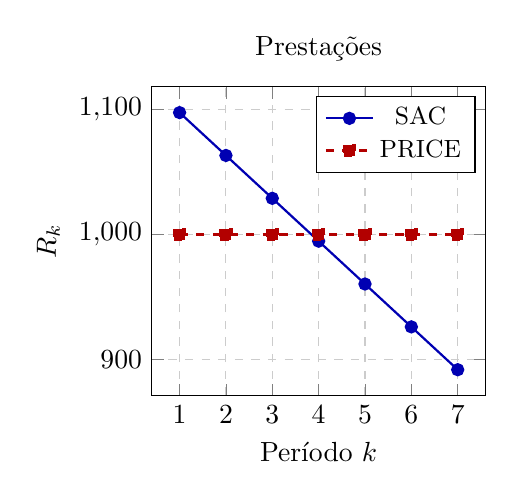
\begin{tikzpicture}
\begin{axis}[
  width=0.48\textwidth, height=5.5cm,
  xlabel={Período $k$}, ylabel={$R_k$},
  title={Prestações},
  legend pos=north east, legend style={font=\small},
  grid=major, grid style={dashed, gray!40},
  xtick={1,2,...,7},
]
  \addplot[thick, color=blue!70!black, mark=*]
    coordinates {(1,1097.64)(2,1063.34)(3,1029.04)(4,994.74)(5,960.44)(6,926.14)(7,891.84)};
  \addplot[thick, color=red!70!black, dashed, mark=square*]
    coordinates {(1,1000)(2,1000)(3,1000)(4,1000)(5,1000)(6,1000)(7,1000)};
  \legend{SAC, PRICE}
\end{axis}
\end{tikzpicture}
\hfill
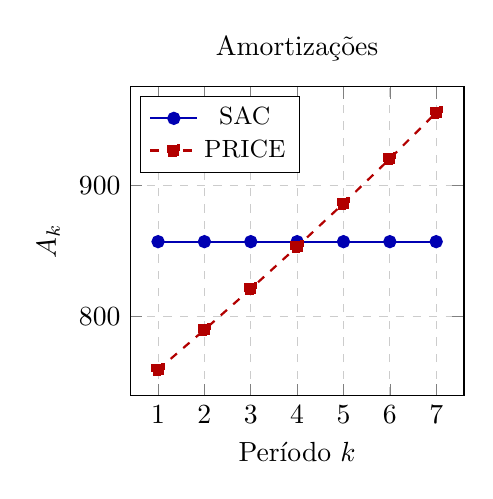
\begin{tikzpicture}
\begin{axis}[
  width=0.48\textwidth, height=5.5cm,
  xlabel={Período $k$}, ylabel={$A_k$},
  title={Amortizações},
  legend pos=north west, legend style={font=\small},
  grid=major, grid style={dashed, gray!40},
  xtick={1,2,...,7},
]
  \addplot[thick, color=blue!70!black, mark=*]
    coordinates {(1,857.14)(2,857.14)(3,857.14)(4,857.14)(5,857.14)(6,857.14)(7,857.14)};
  \addplot[thick, color=red!70!black, dashed, mark=square*]
    coordinates {(1,759.44)(2,789.89)(3,821.14)(4,853.25)(5,886.31)(6,920.39)(7,955.58)};
  \legend{SAC, PRICE}
\end{axis}
\end{tikzpicture}
\end{center}

\paragraph{Síntese:}
\begin{itemize}
  \item \textbf{SAC}: amortiza saldo mais depressa $\Rightarrow$ maior parcela inicial, velocidade de $A_t$ maior e total de juros menor.
  \item \textbf{PRICE}: parcelas iguais facilita o orçamento; juros maiores no total, pois o saldo devedor diminui mais lentamente.
  \item \textbf{Qual escolher?} Depende da preferência intertemporal do devedor. Para quem vai \emph{pré-pagar}, o SAC é mais vantajoso (saldo cai mais rápido).
\end{itemize}

\begin{moderno}[title={PRICE vs.\ SAC no Financiamento Imobiliário FGTS (2025)}]
Financiamento de R\$\,400.000 em 360 meses, taxa de $8{,}16\%$ a.a. (FGTS -- referência 2025):
$i = (1{,}0816)^{1/12}-1 \approx 0{,}6559\%$ a.m.

\medskip
\textbf{PRICE:} $\bar{R} \approx \text{R\$\,}3.006/\text{mês}$; total pago $\approx \text{R\$\,}1.082.160$.

\medskip
\textbf{SAC:} $\bar{A} = 400.000/360 \approx \text{R\$\,}1.111/\text{mês}$ (amortização);
  $1^\text{a}$ prestação $\approx \text{R\$\,}3.737$; $360^\text{a}$ prestação $\approx \text{R\$\,}1.118$;
  total pago $\approx \text{R\$\,}882.000$.

\medskip
O SAC economiza $\approx$ R\$\,200.000 em juros, mas exige capacidade de pagamento maior
nos primeiros anos. Bancos no Brasil oferecem ambos os sistemas.
\end{moderno}
